\documentclass{article}
\usepackage{graphicx}
\usepackage{hyperref}

\usepackage[style=apa, maxcitenames=2]{biblatex} %Imports biblatex package
\addbibresource{references.bib} %Import the bibliography file


\title{My first LaTeX document}
\author{Hubert Farnsworth\thanks{Funded by the Overleaf team.}}
\date{12-12-2022}

\begin{document}

% Title
\maketitle
% TOC
\tableofcontents


\section{Section 1: My First Section}

some text for explaining this section.

\subsection{Text Style}

Normal text

\textbf{Bold text}

\textit{Italic text}

\underline{underline}

Emphasizing

Normal sentence \emph{emph}.

\textit{Italic sentence \emph{emph}.}

\textbf{Bold sentence \emph{emph}.}

\subsection{Figure}

Refer to figure~\ref{fig:brainlab-logo}

\begin{figure}[ht!]
    \centering
    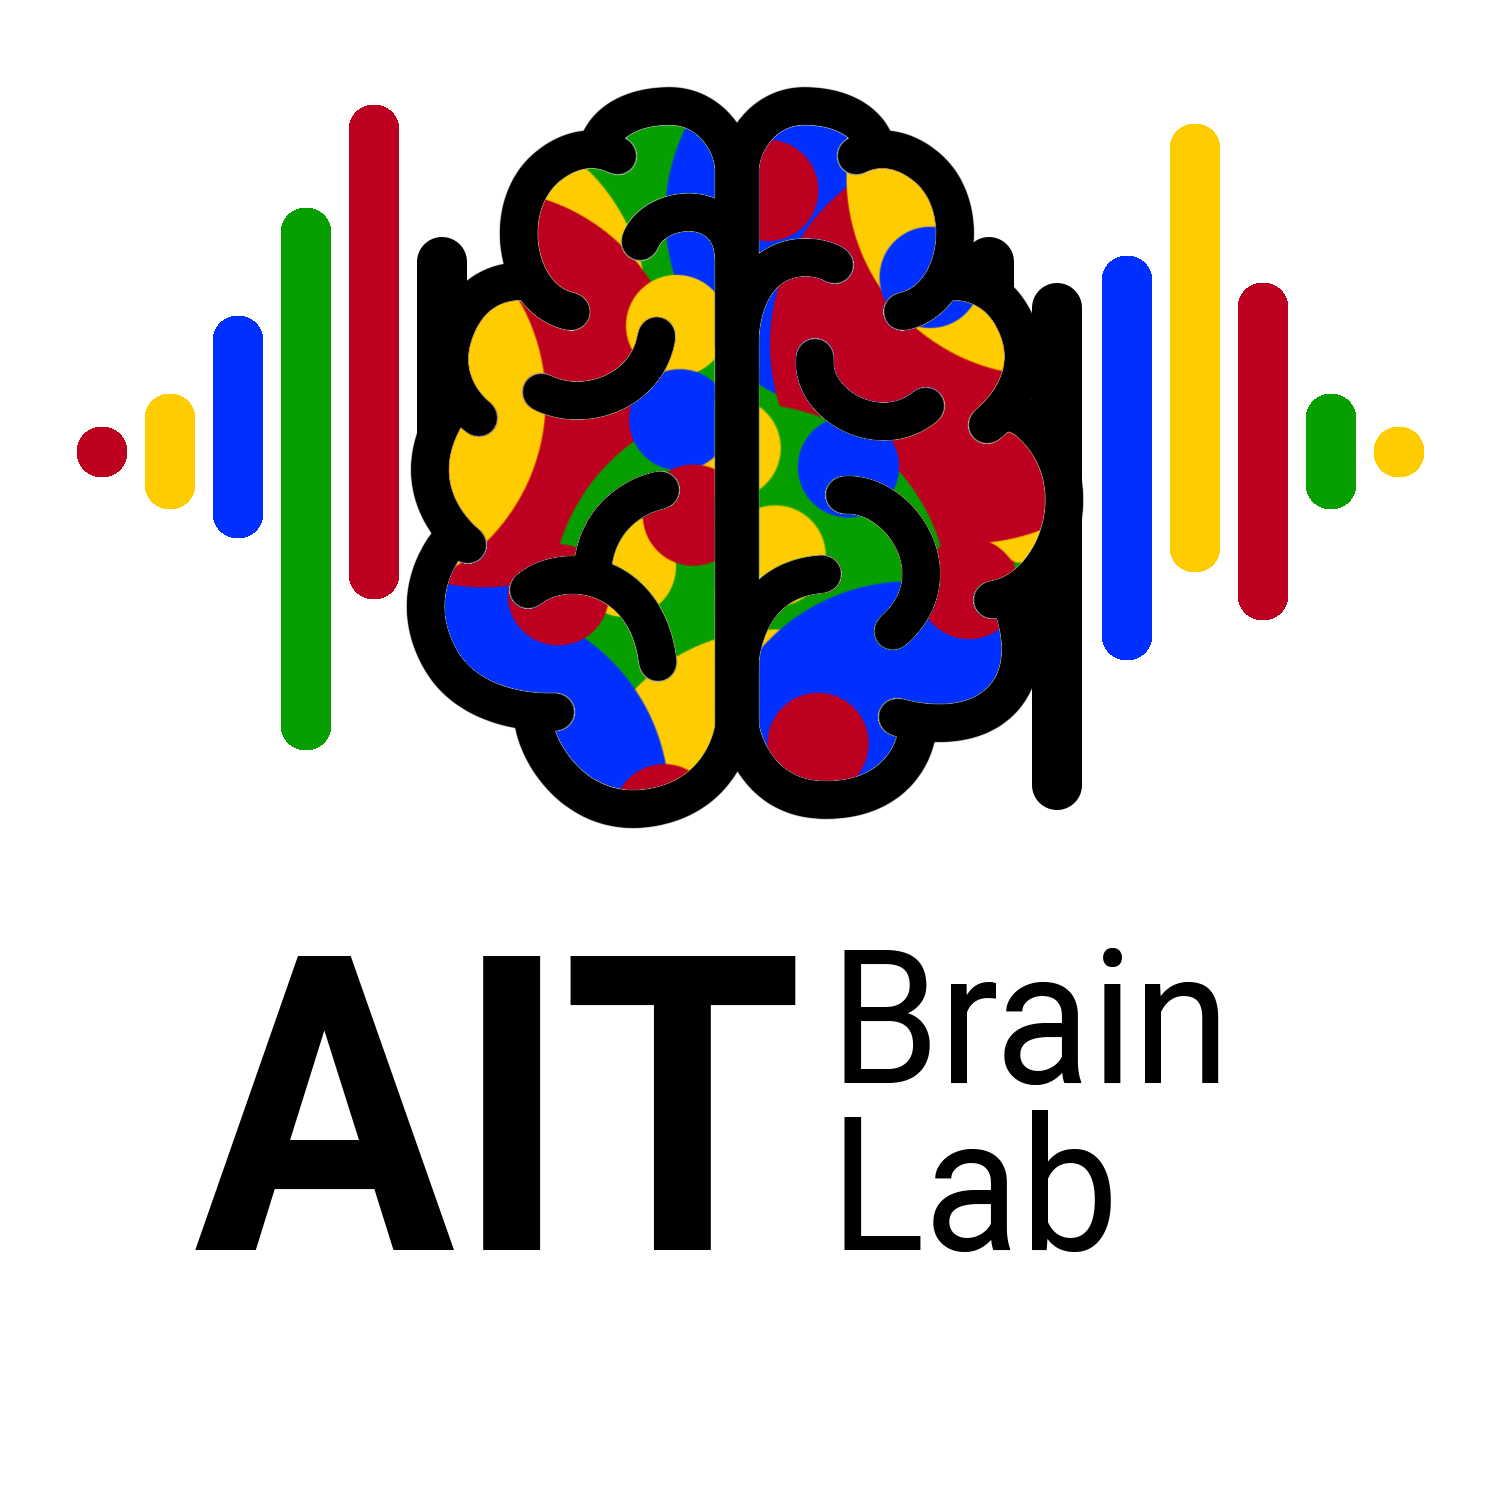
\includegraphics[width=0.75\textwidth]{../4_figure/figures/bci-logo.png}
    \caption{\label{fig:brainlab-logo}AIT Brainlab Logo}
\end{figure}


\subsection{Table}

Refer to table~\ref{tab:demo-table}

\begin{table}[ht!]
    \begin{center}
        \begin{tabular}{||c c c c||} 
        \hline
        Col1 & Col2 & Col2 & Col3 \\ [0.5ex] 
        \hline\hline
        1 & 6 & 87837 & 787 \\ 
        \hline
        2 & 7 & 78 & 5415 \\
        \hline
        3 & 545 & 778 & 7507 \\
        \hline
        4 & 545 & 18744 & 7560 \\
        \hline
        5 & 88 & 788 & 6344 \\ [1ex] 
        \hline
        \end{tabular}
    \caption{\label{tab:demo-table}Your caption.}
    \end{center}
\end{table}



For the master students, 1 paper. For  Ph.D. students, 3 papers. OK? \cite{bcilab}

\subsection{Subject Form}

This form use author as subject.

\begin{itemize}
    \item \textcite{bcilab} asks master and Ph.D. students to publish 1 paper and 3 papers repectivly.
    \item \textcite{2author} -- this is how the 2 authors look like
    \item \textcite{3author} -- this is how the 3 authors look like
    \item \textcite{vaswani2017attention} -- many many authors
\end{itemize}

\subsection{Indirect form}

You probably see this more often. It used for citing sentence (where do you know this).

\begin{itemize}
    \item For the master students, 1 paper. For  Ph.D. students, 3 papers. OK? \parencite{bcilab}
    \item For the master students, 1 paper. For  Ph.D. students, 3 papers. OK? \parencite[18-20]{bcilab}
\end{itemize}

\subsection{Multiple Citation}

When one statement is mentioned by many papers.

\begin{itemize}
    \item Ph.D. must publish 3 papers to graduate \parencite{bcilab,2author,3author}.
    \item \textcite{2author, 3author} mentioned that brainlab is where they work everyday.
\end{itemize}

% https://www.overleaf.com/learn/latex/Bibliography_management_in_LaTeX
\printbibliography %Prints bibliography

\end{document}